\documentclass[11pt, a4paper]{article}
\usepackage[slantfont, boldfont]{xeCJK}
\usepackage{ulem}
\usepackage{amsmath}
\usepackage{booktabs}
\usepackage{colortbl}
\usepackage{fancyvrb}
\usepackage{multirow}
\usepackage[top = 1.0in, bottom = 1.0in, left = 1.0in, right = 1.0in]{geometry}

\setCJKmainfont{SimSun}
\setCJKmonofont{SimSun}

\setlength{\parskip}{0.5\baselineskip}
\setlength{\parindent}{2em}

\title{USACO. Safe Travel}
\author{VFleaKing}

\begin{document}
\maketitle

\section*{题目描述}
小魔怪时常在农场出没。这些讨厌而丑陋的童话里的生物喜欢阻挠从谷仓(即$1$号牧场)走到其它牧场的牛群。牛群中,编号为$i$的牛会从$1$号牧场走到$i$号牧场。每个小魔怪都很有个性,$i$号小魔怪知道$i$号牛一般会沿最短路走到$i$号牧场,于是会在到$i$号牧场的最短路上的最后一条道路中间等着$i$号牛伺机骚扰$i$号牛。

当然,每只牛都不愿意被骚扰,所以想选择一条稍微不同一点的从$1$号牧场(谷仓)到$i$号牧场的路径。

请你对于每只牛$i$求出到达$i$号牧场而不会撞见在$1$号牧场到$i$号牧场的最短路上的最后一条道路上等着的$i$号小魔怪的最短时间。

和平常一样,$m$条双向道路从$1$到$m$编号,$n$个牧场从$1$到$n$编号。第$i$条道路连接$a_i$号牧场和$b_i$号牧场,走过这条路需要$t_i$的时间。没有重边和自环。除此之外,保证对于每个牧场$i$,从$1$号牧场到$i$号牧场的最短路存在且唯一。

举个例子。考虑下面的这些牧场、道路、时间:

\begin{figure}[h]
\centering
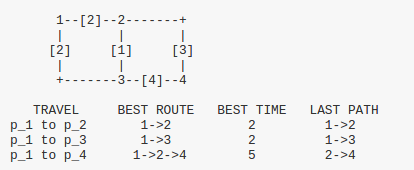
\includegraphics[scale=0.5]{a.png}
\end{figure}

当小魔怪进入农场后:

\begin{figure}[h]
\centering
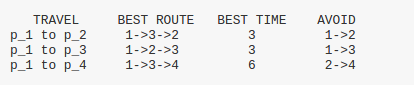
\includegraphics[scale=0.5]{b.png}
\end{figure}

\section*{输入格式}
第一行两个用空格隔开的正整数$n, m$。

接下来$m$行,每行三个正整数表示$a_i, b_i, t_i$。

\section*{输出格式}
输出$n - 1$行,第$i$行包含一个整数表示$i + 1$号牛不撞见$i + 1$号小魔怪的情况下到达$i + 1$号牧场的最快时间。如果不存在这样的路,请输出$-1$。

\section*{样例}
\begin{Verbatim}[frame=single, label=input]
4 5
1 2 2
1 3 2
3 4 4
3 2 1
2 4 3

\end{Verbatim}

\begin{Verbatim}[frame=single, label=output]
3
3
6

\end{Verbatim}

\section*{数据范围}
对于20\%的数据,$n \leq 100$。

对于30\%的数据,$n \leq 400$。

对于60\%的数据,$n \leq 3000$。

对于100\%的数据,$n \leq 100000, m \leq 200000, 1 \leq t_i \leq 1000$。

时间限制:$1\text{s}$

空间限制:$64\text{MB}$

\section*{题解}
\subsection*{算法一}
直接根据题意进行暴力。首先用Floyd $O(n^3)$暴力求出最短路以及最后一条边,然后对于每个$i$,尝试删掉最后一条边然后再跑一次$O(n^3)$的Floyd,就可以求得答案。

时间复杂度$O(n^4)$。可以获得20分。

\subsection*{算法二}
算法一太过暴力了,我们可以很简单地把Floyd改为$O(n^2)$的Dijkstra,那么时间复杂度就可以变为$O(n^3)$。可以获得30分。

\subsection*{算法三}
首先做一次最短路算法求出最短路树。用$d_v$表示到$v$的最短路长度。

由于不能经过最后一条边,所以相当于说去掉最短路树上的父亲边,问最短路。

易知,这样的最短路一定形如$1 \rightarrow v \rightarrow u \rightarrow i$。其中,$v$不在$i$的子树内,$u$在$i$的子树内。$1 \rightarrow v$走的是最短路,$v \rightarrow u$是一条非最短路树上的边,$u \rightarrow i$ 走的是最短路。而这中间的“最短路”一定是我们最短路树上的路径,而且还是直上直下的路径(即路径两端的点的LCA一定是路径两端的点之一)。若非树边$(v, u)$的长度为$w$,则这条路长度为$d_v + w + (d_u - d_i)$。

我们可以对于每个非树边计算对答案的贡献。对于一条非树边$(v, u, w)$,求出$v$与$u$的最近公共祖先$a$。那么对于$v$到$a$的路径上的点$i$(包括$v$但不包括$a$),都应该用$d_u + w + d_v - d_i$进行更新,(当然,还得反着变成$(u, v, w)$再来一次)。这一步暴力就可以了。

于是我们就得到了一个$O(n^2)$的算法,可以获得60分。


\subsection*{算法四}
我们可以用堆优化的Dijkstra算法来求最短路,这样时间复杂度降为了$O((n + m) \log{n})$。于是瓶颈在于后面部分。

我们可以对最短路树进行一次dfs,保存递归栈。当我们到达一个结点$v$时,我们扫与$v$有关的非树边$(v, u, w)$,用倍增算法求出$v$和$u$的最近公共祖先$a$。那么意味着我们要更新$v$到$a$之间的所有点(包括$v$不包括$a$)。注意到这是递归栈的一个连续的区间,可以每次用线段树维护$d_v + w + d_u$的最小值,最后一个结点退栈时查询当前位置的最小值然后减去$d_i$即可。

这样我们就得到了一个 $O((n + m) \log n)$ 的算法。可以获得100分。

当然还有其它算法,可以直接裸上树链剖分、Link-Cut Tree什么的来进行路径上的更新,也是可以获得100分的。

\end{document}
